\subsection{Class diagram di design}
    \begin{flushleft}
        Verranno di seguito riportati i class diagram di design, che ora rispecchiano l'architettura del sistema e tutte le funzionalità nella loro
        interezza. \\
        \emph{\textbf{Nota}}: Tutti i costruttori banali (senza argomenti) e i getter e setter sono stati omessi per rendere più leggibili 
        i diagrammi
    \end{flushleft}

    \subsubsection{Login}
        \begin{figure}[H]
            \centering
            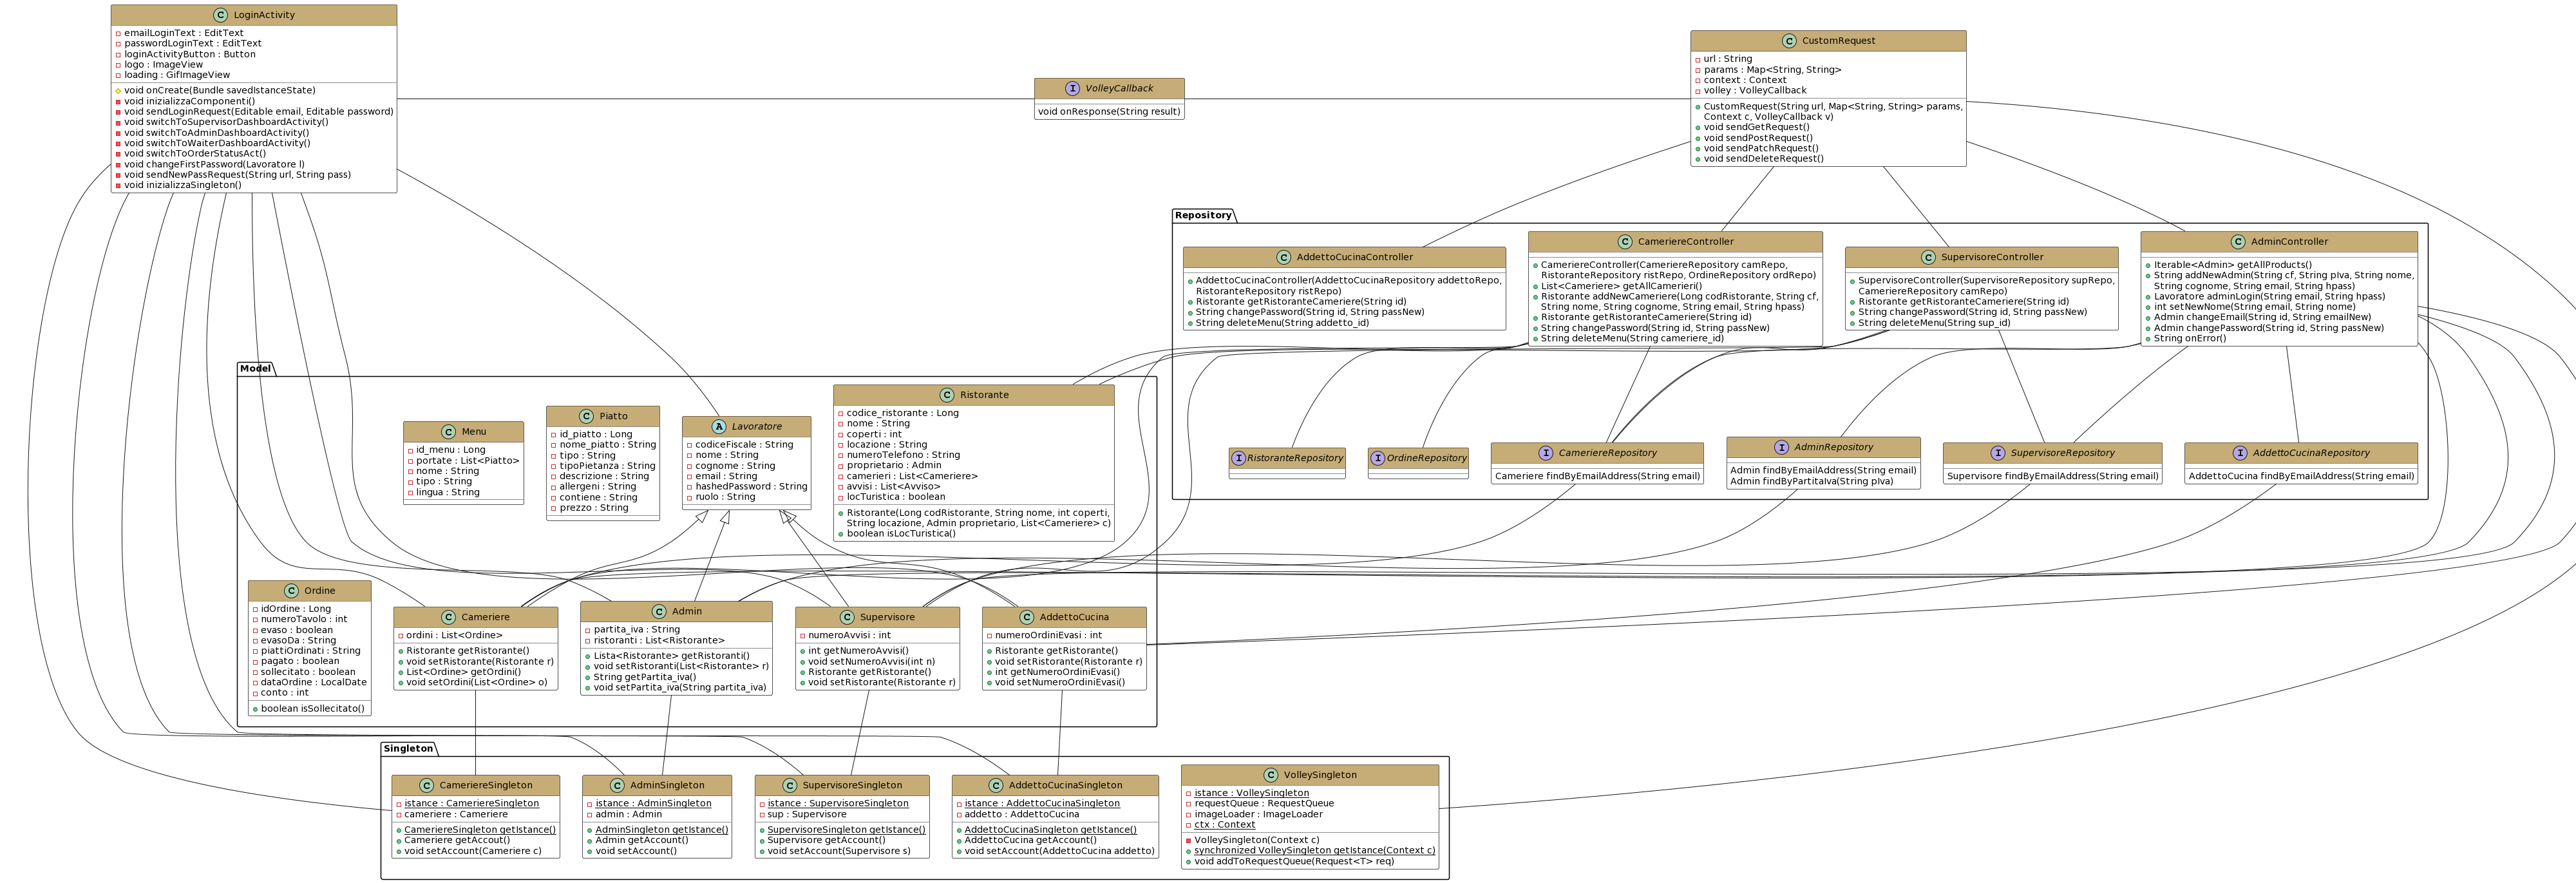
\includegraphics[scale=0.12]{assets/diagrammi/Class diagram di design/ClassDiagram_Login.png}
            \caption*{\textbf{CD01}: Class diagram Login}\label{fig:ClassDiagram_Login}
        \end{figure}
    
    \subsubsection{Gestione piatti}
        \begin{figure}[H]
            \centering
            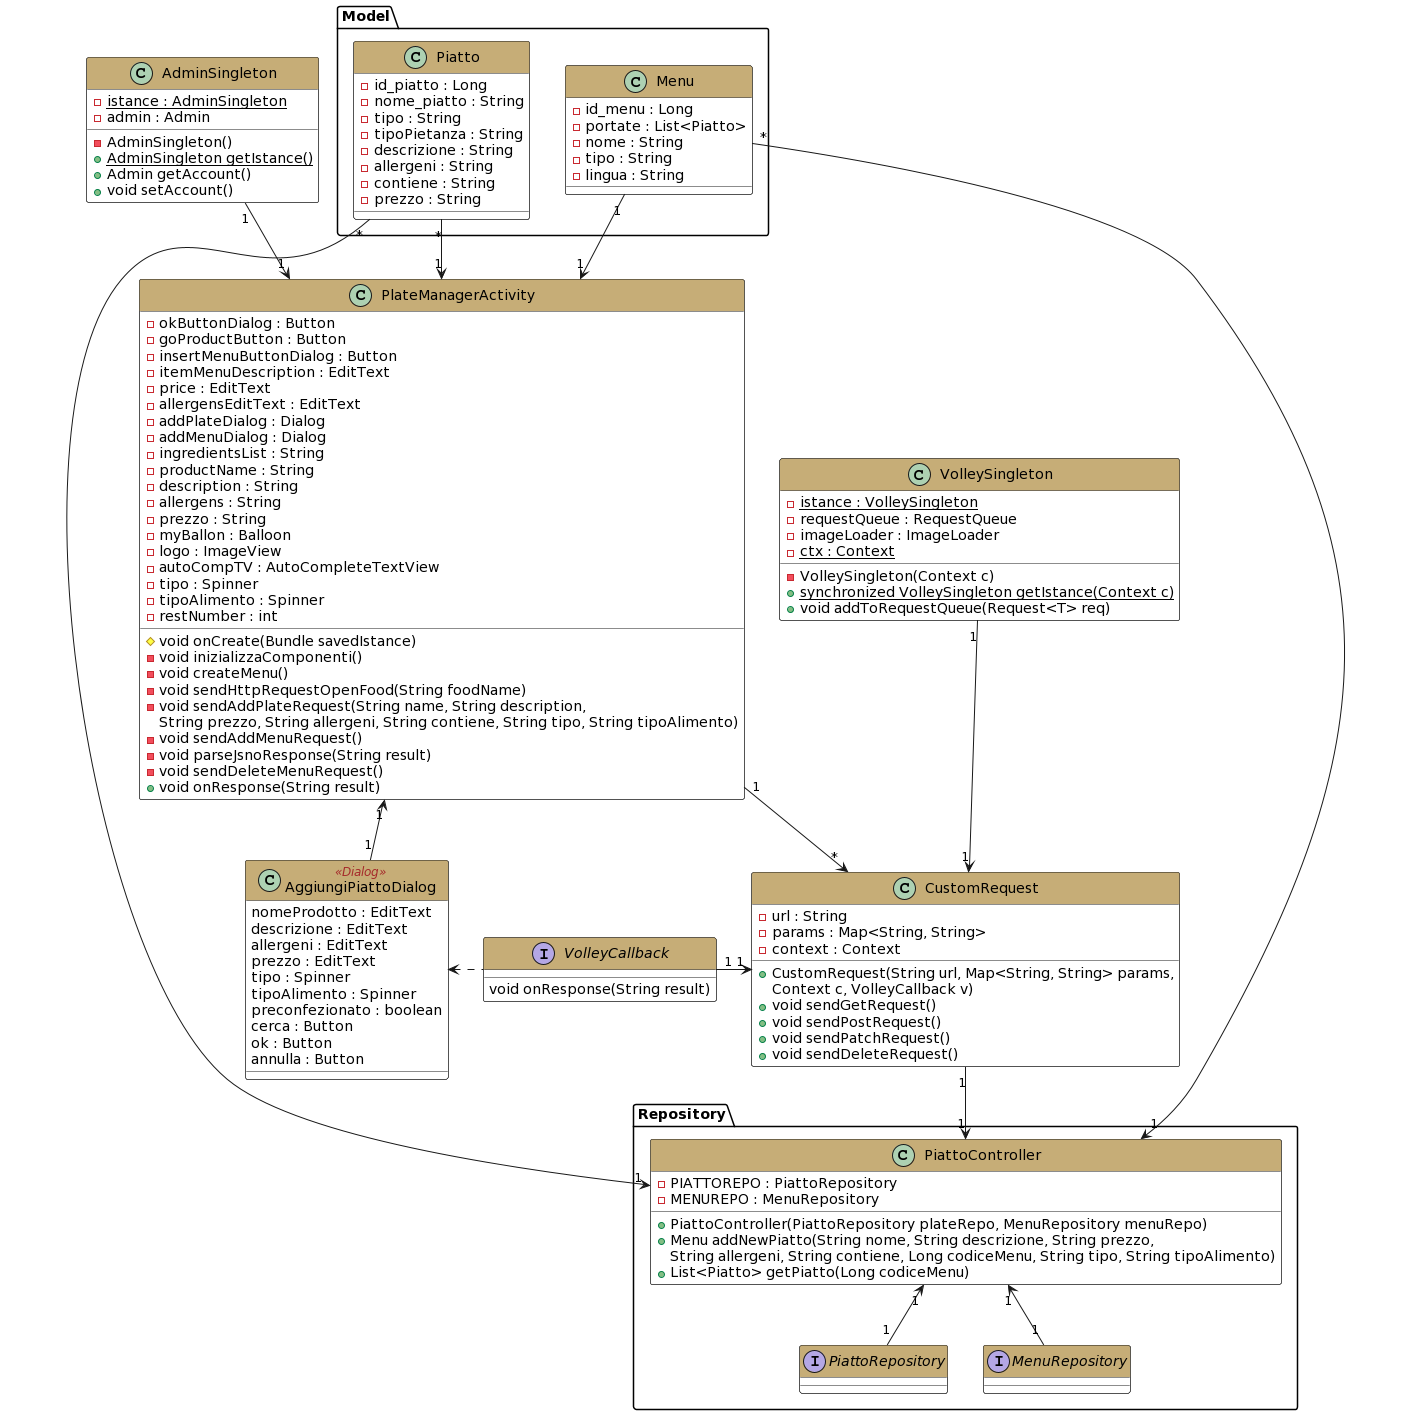
\includegraphics[scale=0.25]{assets/diagrammi/Class diagram di design/gestione piatti.png}
            \caption*{\textbf{CD02}: Class diagram gestione piatti}\label{fig:ClassDiagram_ManagePlates}
        \end{figure}

    \subsubsection{Gestione Avvisi}
        \begin{figure}[H]
            \centering
            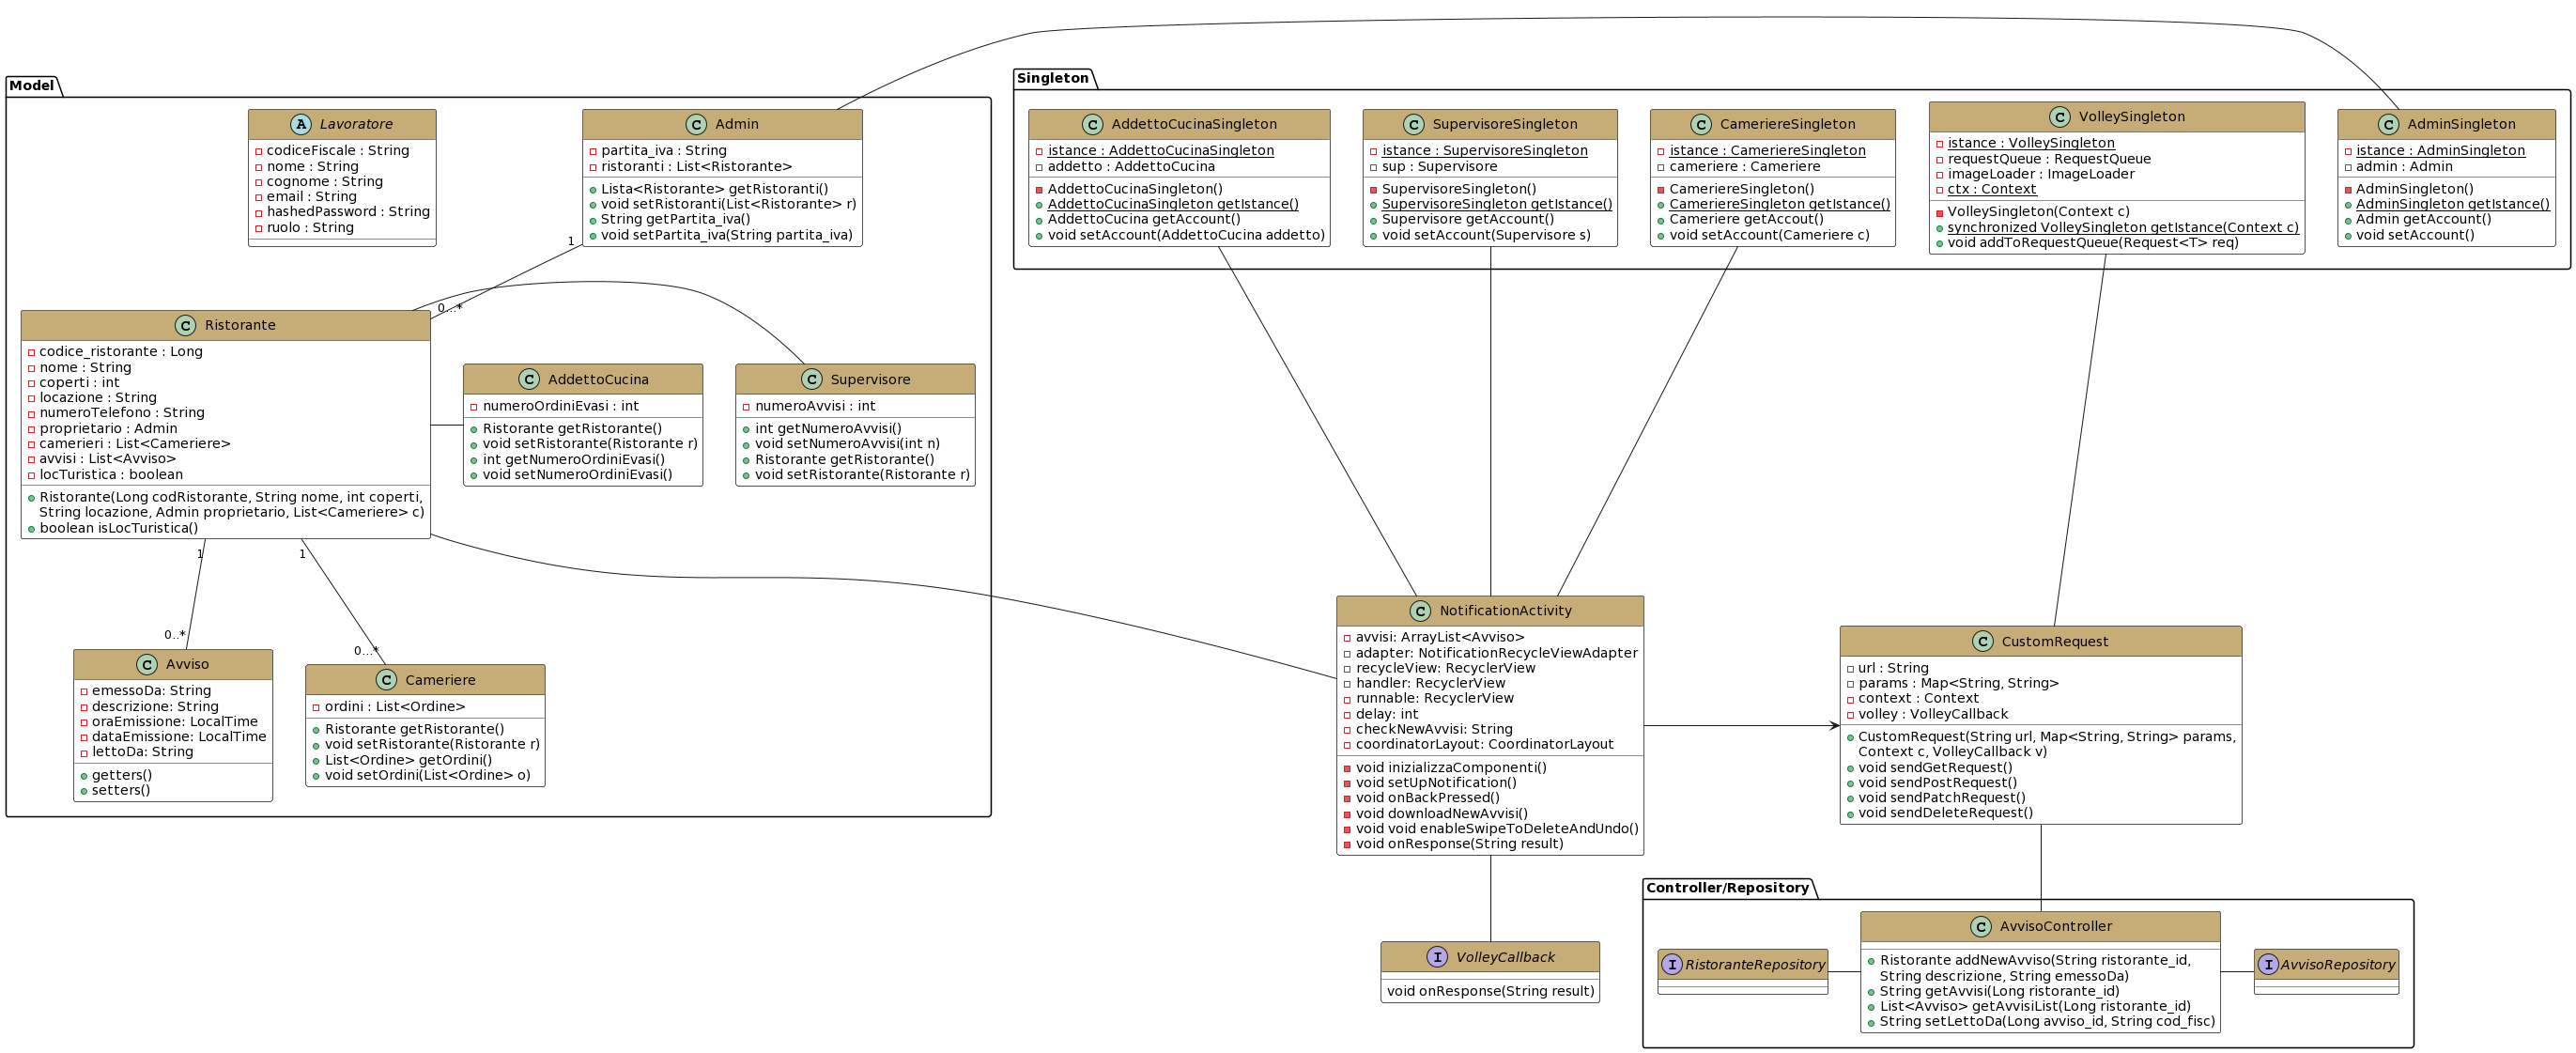
\includegraphics[scale=0.15]{assets/diagrammi/Class diagram di design/ClassDiagramGestioneAvvisi.png}
            \caption*{\textbf{CD03}: Class diagram gestione avvisi}\label{fig:ClassDiagram_ManageAdv}
        \end{figure}
    
    \subsubsection{Gestione Ordini}
        \begin{figure}[H]
            \centering
            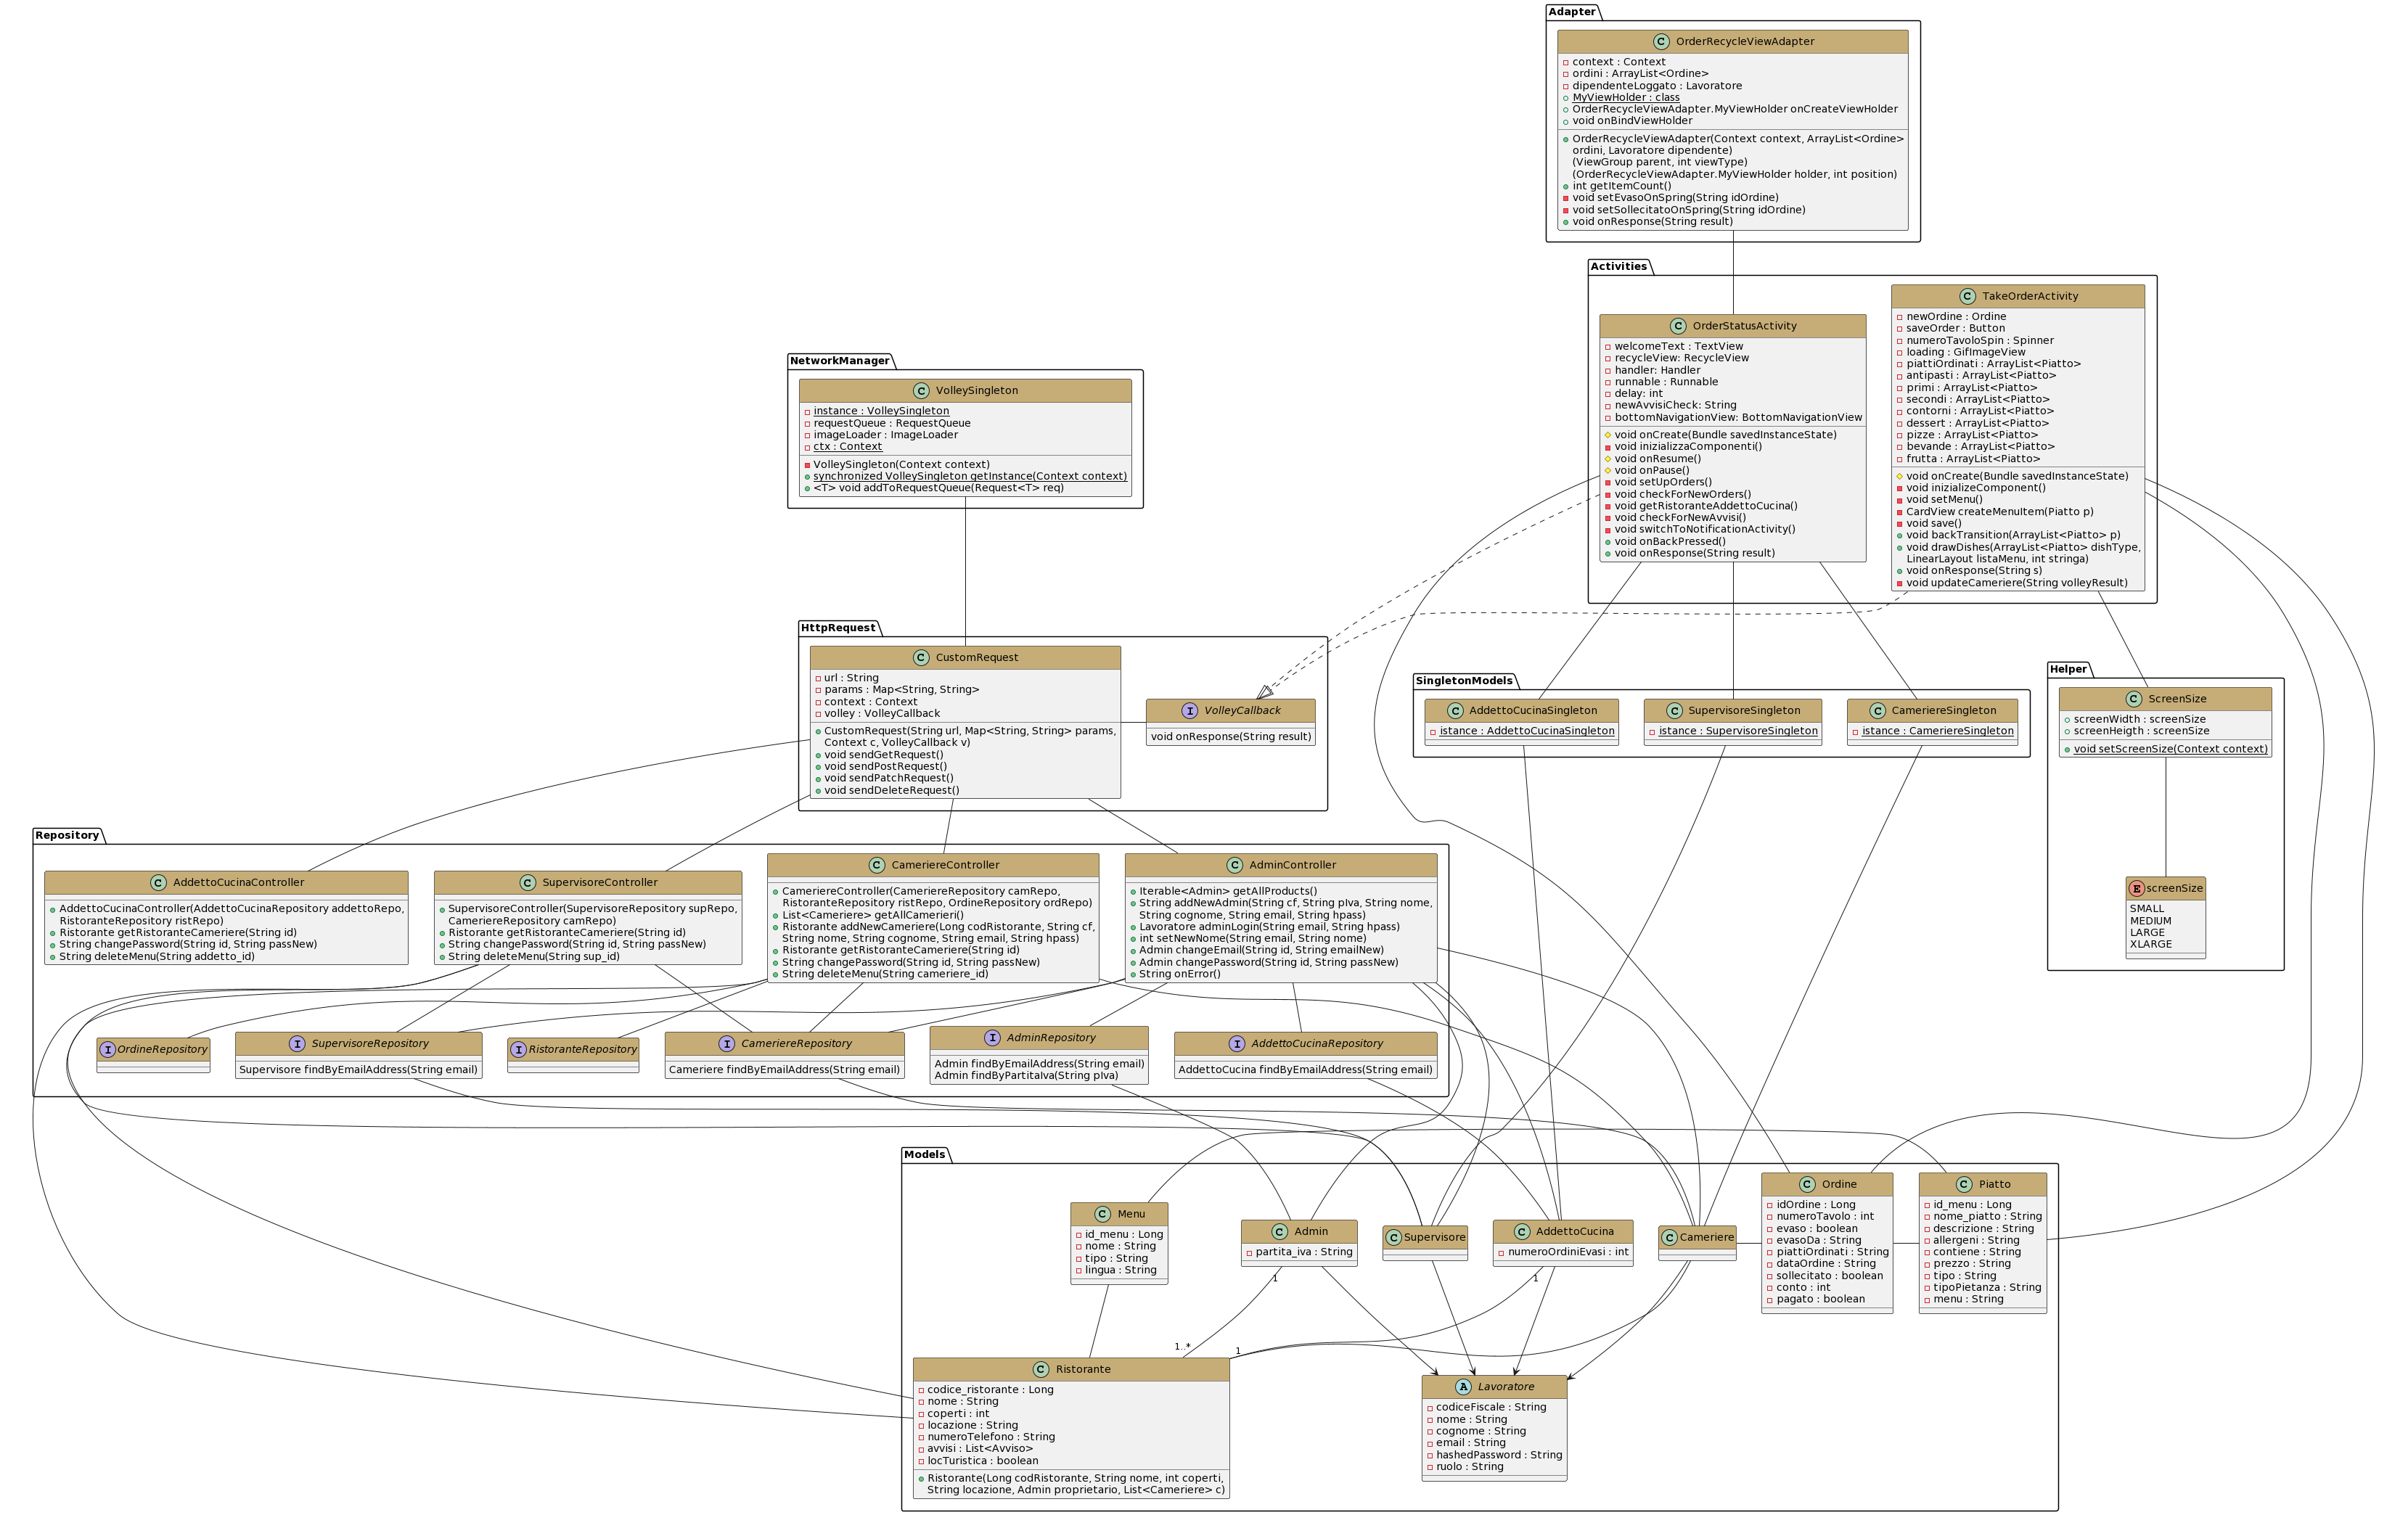
\includegraphics[scale=0.15]{assets/diagrammi/Class diagram di design/Class Diagramm Design Gestione Ordini.png}
            \caption*{\textbf{CD04}: Class diagram gestione ordini}\label{fig:ClassDiagram_ManageOrders}
        \end{figure}

